\chapter{2012年期末试题}
\section{选择题}
\exercise{1}
质点以速度$v=4+t^2 m/s$作直线运动,沿质点运动直线作OX轴,并已知$t=3$s时,质点位于$x=9$m处,则该质点的运动学方程为:
\optionss{x=3t}
{x=4t+\dfrac{1}{2}t^2}
{x=4t+\dfrac{1}{3}t^3-12}
{x=4t+\dfrac{1}{3}t^3+12}

\exercise{2}
力$\vec{F}=3\vec{i}+5\vec{J}$(N),其作用点的位置矢量为$\vec{r}=4\vec{i}-3\vec{j}$(m),则该力对坐标原点
的力矩大小为:
\option{3\textrm{N/m}}{29\textrm{N/m}}{19\textrm{N/m}}{3\textrm{N/m}}

\exercise{3}一特殊弹簧,弹性力 $F=-kx^3$,$k$为劲度系数,$x$为形变量。现将弹簧水平放置于光滑的平面上,一端固定,一端与质量为$m$的滑块相连而处于自然状态,今沿弹簧长度方向给滑块一个冲量,使其获得一速度$v$,则弹簧压缩的最大长度为:
\option{{{\left(\dfrac{4mv}{k}\right)}^{\frac{1}{4}}}}
{{\left(\dfrac{2mv^2}{k}\right)}^{\frac{1}{4}}}
{v\sqrt{\dfrac{k}{m}}}
{v\sqrt{\dfrac{m}{k}}}

\exercise{4}
一根质量为$m$,长为$l$的细而均匀的棒,其下端绞接在水平地板上并竖直的立起,如让它掉下(如图1.1a),则棒将以角速度$ω$撞击地板,如果将同样的棒截成长为$\dfrac{l}{2}$的一段,初始条件不变,则它撞击地板时的角速度最接近于
\option{2\omega}
{\sqrt{2}\omega}
{\omega}
{\frac{\omega}{\sqrt{2}}}
\begin{figure}[!h]
	\centering
	\subfigure[选择4 示意图]{
	\begin{minipage}[t]{0.3\linewidth}
		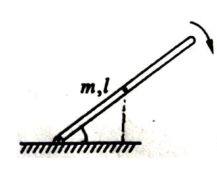
\includegraphics[width=\textwidth]{./illus/2012_1.png}
	\end{minipage}}
	\quad
	\subfigure[选择8 示意图]{
		\begin{minipage}[t]{0.3\linewidth}
		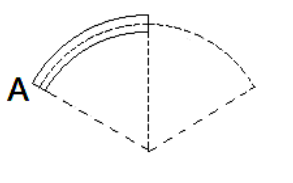
\includegraphics[width=\textwidth]{./illus/2012_2.png}
	\end{minipage}}
	\quad
	\subfigure[选择9 示意图]{
	\begin{minipage}[t]{0.3\linewidth}
		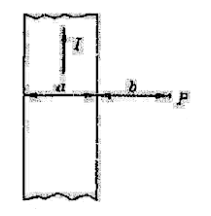
\includegraphics[width=\textwidth]{./illus/2012_3.png}
	\end{minipage}}
	\caption{三张题图}
\end{figure}
\exercise{5}
关于狭义相对论,下列几种说法中叙述\CJKunderdot{错误}的是:
\options{一切运动物体的速度都不能大于真空中的光速}
{在任何惯性系中,光在真空中沿任何方向的传播速率都相同}
{在真空中,光的速度与光源的运动状态无关}
{在真空中,光的速度与光的频率有关}

\exercise{6}两个均匀带电的同心球面,半径分别为$R_1,R_2(R_1<R_2)$,小球面带电$Q$,大球面带电$-Q$,下列各图中正确表示了电场分布的是
\begin{figure}[!h]
	\centering
	\option
	{\subfigure{
		\begin{minipage}[t]{\linewidth}
			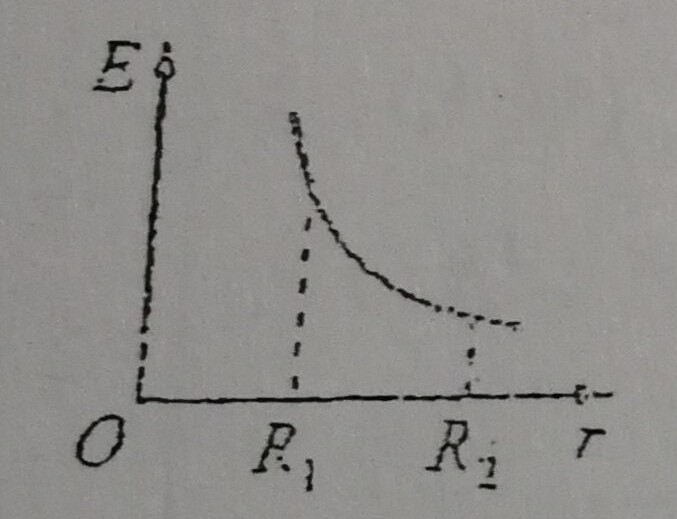
\includegraphics[width=\textwidth]{./illus/2012_4a.jpg}
	\end{minipage}}}
	{\subfigure{
		\begin{minipage}[t]{\linewidth}
			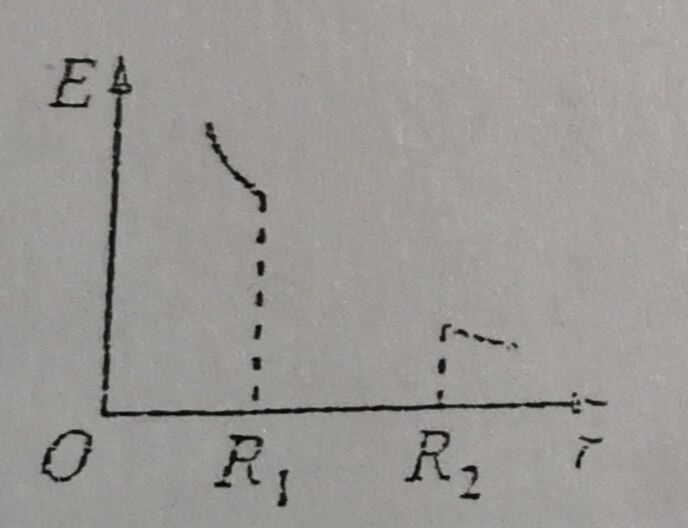
\includegraphics[width=\textwidth]{./illus/2012_4b.jpg}
	\end{minipage}}}
	{\subfigure{
		\begin{minipage}[t]{\linewidth}
			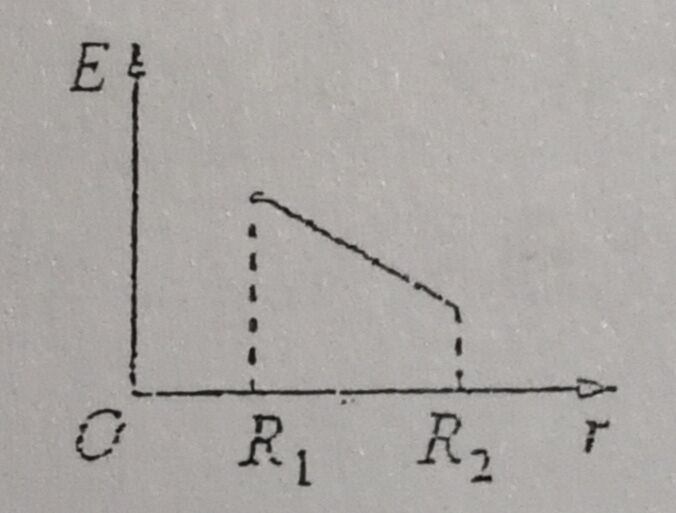
\includegraphics[width=\textwidth]{./illus/2012_4c.jpg}
	\end{minipage}}}
	{\subfigure{
	\begin{minipage}[t]{\linewidth}
		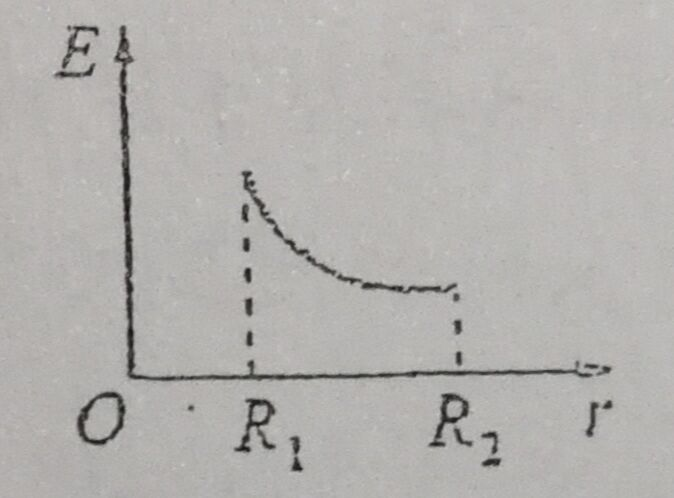
\includegraphics[width=\textwidth]{./illus/2012_4d.jpg}
	\end{minipage}}}
	\caption{选择6}
\end{figure}

\exercise{7}
磁场的高斯定理$\oiint\vec{B}\cdot\vec{S}=0$说明了下面表述正确的是:
\options{穿入闭合曲面$S$的磁感应线条数必然等于穿出的磁感应线条数}{穿入闭合曲面$S$的磁感应线条数不等于穿出的磁感应线条数}{一根磁感应线可以终止在闭合曲面$S$内}{一根磁感应线不可能完全处于闭合曲面$S$内}

\exercise{8}
有一均匀带电的绝缘体细圆弧,其圆心角为$\dfrac{2}{3}\pi$,测得其圆心$O$处的电场强度大小为$E_0$,今将此圆弧对折,如图,则$O$点电场强度大小为
\option{\dfrac{E_0}{2}}
{2E_0}
{\dfrac{\sqrt{3}}{3}E_0}
{\dfrac{2\sqrt{3}}{3}E_0}        

\exercise{9}
如图所示,有一无限长通有电流的薄平直铜片,宽度为$a$,厚度不计,电流$I$在铜片上均匀分布,在铜片外与铜片共面,离铜片右边缘为$b$处的$P$点的磁感应强度$\vec{B}$大小为
\optionss{\dfrac{\mu_0I}{2\pi(a+b)}}
{\dfrac{\mu_0I}{2\pi a}\ln\dfrac{a+b}{b}}
{\dfrac{\mu_0I}{2\pi b}\ln\dfrac{a+b}{a}}
{\dfrac{\mu_0I}{2\pi(\frac{a}{2}+b)}}%此处原题处多了个a

\exercise{10}
对位移电流,有下列四种说法,请指出哪一种说法正确
\options{位移电流是由变化的电场产生的\footnote{笔者认为此处说法不准确,应是“位移电流是变化的电场的一种等效”。详见参考答案。}}
{位移电流是由线性变化的磁场产生的}
{位移电流产生焦耳热}
{位移电流的磁效应不服从安培环路定理}

\section{填空题}

\exercise{1}
质量为$m$的物体,初速极小,在外力作用下从原点起沿x轴正向运动,所受外力方向沿x轴正向,大小为$F=kx$。物体从原点运动到坐标为$x_0$点的过程中所受外力冲量的大小为\ul。
%为什么初速极小

\exercise{2}
如图所示,一条轻质细绳绕过一个半径为$R$,转动惯量为$mR^2$的定滑轮(轮轴光滑),一端系着一个质量为 $2m$的物体,另一端有质量为$4m$的人抓住绳子相对于绳子匀速向上爬,则物体的加速度大小为\ul;若人相对于地面匀速向上爬,则物体的加速度大小为\ul。
\begin{figure}[!h]
	\centering
	\subfigure[填空2 示意图]{
		\begin{minipage}[t]{0.3\linewidth}
			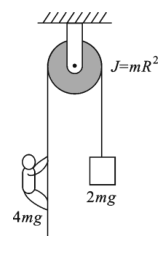
\includegraphics[width=\textwidth]{./illus/2012_5.png}
	\end{minipage}}
	\quad
	\subfigure[填空5 示意图]{
		\begin{minipage}[t]{0.5\linewidth}
			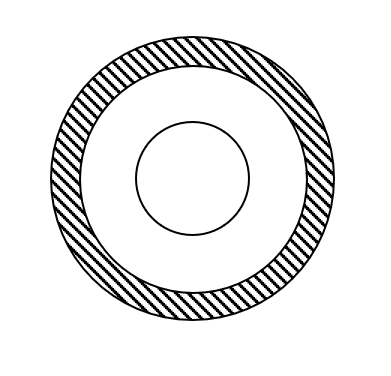
\includegraphics[width=\textwidth]{./illus/2012_6.ai}
	\end{minipage}}
	\caption{两张题图}
\end{figure}

\exercise{3}
一个人站在转动的转台中央,在他伸出的两个手中各握有一个重物,若此人向着胸部缩回他的双手及重物,忽略所有摩擦,则系统的转动惯量\ul,系统的转动角速度\ul,系统的角动量\ul ,系统的转动动能\ul。(填增大、减小或不变)

\exercise{4}
设电子的静止质量为$m_0$,将一个电子从静止加速到速率为$0.6c$($c$为真空中光速),需做功\ul。在速度$v=$\ul 的情况下电子的动能等于它的静止能量。

\exercise{5}
如图所示,一带电荷量为$q$,半径为$r_A$的金属球$A$,与一原先不带电、内外半径分别为$r_B$和$r_C$的金属球壳$B$同心放置。则图中$P$点的电场强度大小$E=$\ul。如果用导线将$A,B$连接起来,则$A$球的电势 $U=$\ul。(设无穷远处电势为零)

\exercise{6}
两块无限大的均匀带电平行平板,其电荷面密度分别为$\sigma$及$-2\sigma$,如图所示,试写出各区域的电场强度$\vec{E}$的大小:1区$\vec{E}$的大小\ul;2区$\vec{E}$的大小\ul;3区$\vec{E}$的大小\ul。

\exercise{7}
同种材质、粗细均匀的载流导线在平面内分布,弯成如图所示形状。导线中通有电流为$I,I_1,I_2$。它们在点$O$的磁感应强度\CJKunderdot{大小}为(用含$I_1,I_2$的式子表示)\ul;代入$I_1,I_2$大小关系可得磁感应强度大小为\ul。

\begin{figure}[!h]
	\centering
	\subfigure[填空6 示意图]{
		\begin{minipage}[t]{0.3\linewidth}
			\includegraphics[width=\textwidth]{./illus/2012_7.ai}
	\end{minipage}}
	\quad
	\subfigure[填空7 示意图]{
		\begin{minipage}[t]{0.3\linewidth}
			\includegraphics[width=\textwidth]{./illus/2012_8.ai}
	\end{minipage}}
	\quad
	\subfigure[填空8 示意图]{
		\begin{minipage}[t]{0.3\linewidth}
			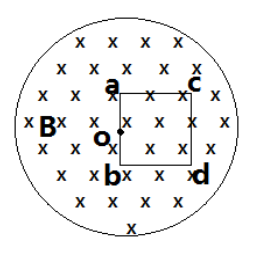
\includegraphics[width=\textwidth]{./illus/2012_9.png}
	\end{minipage}}
	\caption{三张题图}
\end{figure}

\exercise{8}
圆柱形区域内存在一匀强磁场$B$,且以恒定变化率$\dy{B}{t}$减小,一边长为$l$的正方形导体框abcd置于该磁场中,框平面与磁场垂直,圆柱形匀强磁场中心O位于ab的中心,如图所示,则c处有旋电场强度大小$E_c=$\ul ;dc段上的感生电动势大小$\varepsilon_{\textrm{dc}}$=\ul。


\section{解答题}%用\vspace控制答题空间
%\begin{wrapfigure}{1}[r][1em]\end{wrapfigure}
\exercise{1}
如图所示,一根质量均匀分布的细棒长为$L$,质量为$m$。现将细棒放在粗糙的水平桌面上,棒可绕过其端点$O$的竖直轴转动,已知棒与桌面的摩擦系数为$\mu$,棒的初始角速度为$\omega$,试求:%试求的统一格式

\exercisequestion{1}细棒对给定轴的转动惯量;

\exercisequestion{2}细棒绕轴转动时所受到的摩擦力矩;

\exercisequestion{3}细棒从角速度$\omega_0$开始到停止转动所经过的时间。
\begin{figure}[!h]
	\begin{flushright}
		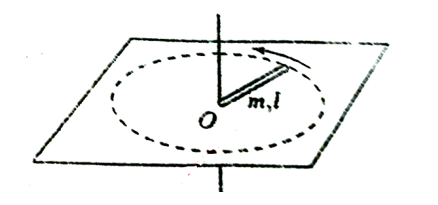
\includegraphics[width=0.4\textwidth]{./illus/2012_10.png}
		\caption{解答1 示意图}
	\end{flushright}
\end{figure}

\exercise{2}
设快速运动的介子的能量约为$E=3000$MeV,而这种介子在静止时的能量$E_0=100$MeV。若这种介子的固有寿命为$\tau_0=2\times 10^{-6}$s,试求:

\exercisequestion{1}介子衰变前运动的距离。

\vspace{10em}
\exercise{3}
电荷分布在半径为$R$的球体内,电荷量体密度为$\rho=\rho_0(1-\dfrac{r}{R})$,式中$\rho_0$为常量,$r$为球心到球内一点的距离,试求:

\exercisequestion{1}球内、球外的电场强度大小;

\exercisequestion{2}电场强度的最大值。

\vspace{10em}
\exercise{4}
如图所示,一无限长直导线$L_1$载有电流$I_1$,旁边有与它垂直且共面的一段导线$L_2$,$L_2$长为$l$,载有电流$I_2$,靠近$L_1$的一端到$L_1$的距离也是$l$,试求:

\exercisequestion{1}$L_1$上的电流作用在$L_2$上的力的大小及方向。
\begin{figure}[!h]
	\begin{flushright}
		\includegraphics[width=0.4\textwidth]{./illus/2012_11.ai}
		\caption{解答4 示意图}
	\end{flushright}
\end{figure}

\exercise{5}
两根无限长的平行输电线,相距为$l$,载有大小相等而方向相反的电流$I=I_0cos\omega t$ ;旁边有一长为$a$,宽为$b$的矩形线圈,它们在同一平面内,长边与输电线平行,到最近一条的距离为$d$,如图所示,试求:

\exercisequestion{1}导线与矩形线圈的互感系数;

\exercisequestion{2}矩形线圈中的感应电动势。
\begin{figure}[!h]
	\begin{flushright}
		\includegraphics[width=0.4\textwidth]{./illus/2012_12.ai}
		\caption{解答5 示意图}
	\end{flushright}
\end{figure}

\newpage
\section{参考答案}
\note 对于解析中没带矢量符号的矢量,认为是在计算其大小,以后不再说明。
\vspace{-2em}
\subsection{选择题和填空题}
\choosing{1}{10} CBBBD DADBA

\filling{\sqrt{mkx_0^2}}
{\dfrac{2}{7}g\quad\dfrac{2}{3}g}
{\text{减小\quad 增大\quad 不变\quad 增大}}
{\dfrac{1}{4}m_0c^2\quad \dfrac{\sqrt{3}}{2}c}
{\dfrac{q}{4\pi\varepsilon_0r^2}\quad\dfrac{q}{4\pi\varepsilon_0r_c}}
{\dfrac{\sigma}{2\varepsilon_0}\quad\dfrac{3\sigma}{2\varepsilon_0}\quad\dfrac{\sigma}{2\varepsilon_0}}
{\dfrac{\mu_0}{4\pi R}|I_1(2\pi-\theta)-I_2\theta|\quad 0}
{\dfrac{\sqrt{5}}{4}l\dy{B}{t}\quad\dfrac{1}{2}l^2\dy{B}{t}}

部分题目解析:

\exerciseanswer{选择}{4}

\tips 光的波长是与频率成反比的,二者之积为光速。不同颜色的光的波速相同。

\exerciseanswer{选择}{8}

\solve 设圆弧初始时电荷线密度为$\lambda$,则后来电荷线密度为$2\lambda$,半径为$R$,两种情况下均以O与圆弧中点连线为极轴,建立坐标系进行积分。
\begin{align*}
	E_0&=\int_{-\frac{1}{3}\pi}^{\frac{1}{3}\pi}\dfrac{1}{4\pi\varepsilon_0}\dfrac{\lambda R\di{\theta}}{R^2}\cos\theta\\
	&=\dfrac{\sqrt{3}\lambda}{4\pi\varepsilon_0R}\\
	E&=\int_{-\frac{1}{6}\pi}^{\frac{1}{6}\pi}\dfrac{1}{4\pi\varepsilon_0}\dfrac{2\lambda R\di{\theta}}{R^2}\cos\theta\\
	&=\dfrac{\lambda}{2\pi\varepsilon_0R}=\dfrac{2}{\sqrt{3}}E_0
\end{align*}
故选D。

\exerciseanswer{选择}{10}

\note A选项说法不准确。麦克斯韦把$\dy{\varPsi}{t}$称为$I_D$,前者的含义就是变化的电场,所以说位移电流就是变化电场的一个替代,为了使“电流生磁”的形式保持不变。若要用“产生”,说明二者应该是独立的两个事物,而事实上并不是。

\exerciseanswer{填空}{1}

\tips 本题综合了动能定理、动量定理、动能和动量的关系,由动能到动量再到冲量,计算简单但融入了较多思想,希望同学们理解、运用。

\exerciseanswer{填空}{2}

\solve 第一种情况,人和轻绳端点(右端物体)的加速度相同,故列式上与把人换成质量为$4m$的重物无异。由角动量定理:
\begin{gather*}
	(4mg-2mg)R=\dy{(4mRv+2mRv+Jw)}{t}=7mR^2\beta\\
	\beta=\dfrac{2}{7}g
\end{gather*}
第二种情况,人对轴的角动量不变,故:
\begin{gather*}
(4mg-2mg)R=\dy{(2mRv+Jw)}{t}=3mR^2\beta\\
\beta=\dfrac{2}{3}g
\end{gather*}

\exerciseanswer{填空}{5}

\tips 导线连接后,二者成为等势体,只考虑球壳外的场强即可。

\exerciseanswer{填空}{7}

\solve 本题是毕奥萨法尔定律的应用。由叉积的性质,两段直导线在$O$处的磁感应强度为0,而对圆导线:
\begin{align*}
	B_1&=\int_{0}^{2\pi-\theta}\dfrac{\mu_0}{4\pi}\dfrac{I_1\di{r}}{R}\\
	&=\dfrac{\mu_0I_1}{4\pi R}(2\pi-\theta)
\end{align*}
同理
\[
	B_2=\dfrac{\mu_0I_2}{4\pi R}\theta
\]
所以第一空应填$\dfrac{\mu_0}{4\pi R}|I_1(2\pi-\theta)-I_2\theta|$
由题,$I_1,I_2$流过的两段导线并联,而其电阻与长度成正比,电流与长度(其对应的圆心角)成反比,代入即得磁感应强度为零。

\exerciseanswer{填空}{8}

\solve 可以在磁场区内部取一半径为$r$的环路,其上每一点都有:
\begin{gather*}
	E_v\cdot 2\pi r=\dy{B}{t}\cdot \pi r^2\\
	E_v=\dfrac{r}{2}\dy{B}{t}
\end{gather*}
方向沿圆周切线。所以第一空填$\dfrac{\sqrt{5}}{4}l\dy{B}{t}$。

\begin{figure}
	\centering
	\includegraphics[width=0.4\textwidth]{./illus/2012_s1.ai}
\end{figure}
如图所示,第二空所求电动势无法在回路中研究,故对感生电场强度积分。
\begin{align*}
	\varepsilon_{\textrm{dc}}&=\int_{-\frac{l}{2}}^{\frac{l}{2}}E_v\cos\theta\di{x}\\
	&=\int_{-\frac{l}{2}}^{\frac{l}{2}}\dfrac{r}{2}\dy{B}{t}\cdot\dfrac{l}{r}\di{x}(r=\sqrt{x^2+l^2})\\
	&=\dfrac{1}{2}l^2\dy{B}{t}
\end{align*}

\subsection{解答题}
\solves{1}%普通格式,英文括号,然后空一下
(1)设细棒外侧端点为$A$。
\begin{align*}
	J&=\int_O^A\di{m\cdot r^2}\\
	&=\dfrac{m}{L}\int_0^Lx^2\di{x}\\
	&=\dfrac{1}{3}mL^2
\end{align*}
(2)
\begin{align*}
	M_f&=\int_O^A|\vec{r}\times\vec{F}|\\
	&=\int_0^Lx\cdot\mu\cdot\dfrac{m}{L}\di{x}g\\
	&=\dfrac{\mu mg}{L}\int_0^Lx\di{x}\\
	&=\dfrac{1}{2}\mu mgL
\end{align*}
方向与棒角动量方向相反(竖直向下)。

(3)
\begin{gather*}
	M_f=J\beta\\
	-\omega_0=0-\beta t
\end{gather*}
则
\[
	t=\dfrac{J\omega_0}{M_f}=\dfrac{2L\omega_0}{3\mu g}
\]

\solves{2}
由题:
\begin{gather*}
	E=mc^2=\dfrac{m_0}{\sqrt{1-{(\frac{v}{c})}^2}}\\
	E_0=m_0c^2
\end{gather*}
则:
\begin{gather*}
	\sqrt{1-{(\frac{v}{c})}^2}=\dfrac{E_0}{E}=\dfrac{1}{30}\\
	v=\dfrac{\sqrt{899}}{30}c
\end{gather*}
而
\[
	\tau=\dfrac{\tau_0}{\sqrt{1-{(\frac{v}{c})}^2}}=30\tau_0
\]
故:
\[
	s=v\tau=\sqrt{899}c\tau_0=1.799\times 10^4\textrm{m}
\]

\solves{3}
(1) 取球心与球体球心重合、半径为$r$的球面高斯面,由高斯定理:
\[
	E\cdot 4\pi r^2=\dfrac{q}{\varepsilon_0}
\]
在球内:
\begin{align*}
	q&=\int_0^r\rho_0(1-\dfrac{r}{R})\cdot 4\pi r^2\di{r}\\
	&=4\pi\rho_0\int_0^r(r^2-\dfrac{r^3}{R})\di{r}\\
	&=4\pi\rho_0(\dfrac{1}{3}r^3-\dfrac{1}{4R}r^4)
\end{align*}
在球外:
\begin{align*}
q&=\int_0^R\rho_0(1-\dfrac{r}{R})\cdot 4\pi r^2\di{r}\\
&=4\pi\rho_0\int_0^R(r^2-\dfrac{r^3}{R})\di{r}\\
&=\dfrac{1}{3}\pi\rho_0R^3
\end{align*}
所以$E=
\begin{cases}
\dfrac{\rho_0}{\varepsilon_0}(\dfrac{1}{3}r-\dfrac{1}{4R}r^2),&r<R\\
\dfrac{\rho_0R^3}{\varepsilon_0r^2},&r>R
\end{cases}$

(2) 由(1),$r>R$时,$E$随$r$的增大而减小;

$r<R$时,由二次函数性质,$r>\dfrac{2}{3}R$时,$E$随$r$的增大而减小,反之相反。

电场强度函数是连续的,所以
\[
	E_{max}=E(\dfrac{2}{3}R)=\dfrac{\rho_0R}{9\varepsilon_0}
\]

\solves{4}
对$I_1$的磁场,\amperecircuitaltheorem{1}
\begin{align*}
	F&=\int_l^{2l}|I\di{\vec{r}}\times \vec{B}|\\
	&=\dfrac{\mu_0I_1I_2}{2\pi}\int_l^{2l}\dfrac{\di{r}}{r}\\
	&=\dfrac{\mu_0I_1I_2\ln 2}{2\pi}
\end{align*}
方向:沿$I_1$的方向。

\solves{5}
(1) \amperecircuitaltheorem{}以垂直于纸面向内(沿线圈顺时针)为正向。
\begin{align*}
	\phi&=\phi_1+\phi_2\\
	&=\int_{d}^{b+d}\dfrac{\mu_0I}{2\pi r}\cdot a\di{r}
	-\int_{d+l}^{b+d+l}\dfrac{\mu_0I}{2\pi r}\cdot a\di{r}\\
	&=\dfrac{\mu_0Ia}{2\pi}(\int_{d}^{b+d}\dfrac{\di{r}}{r}-\int_{d+l}^{b+d+l}\dfrac{\di{r}}{r})\\
	&=\dfrac{\mu_0Ia}{2\pi}\ln\dfrac{(b+d)(d+l)}{d(b+d+l)}
\end{align*}
所以
\[
	M=\dfrac{\phi}{I}=\dfrac{\mu_0a}{2\pi}\ln\dfrac{(b+d)(d+l)}{d(b+d+l)}
\]
(2) 
\begin{align*}
	\varepsilon&=-\dy{\phi}{t}\\
	&=-\dfrac{\mu_0a}{2\pi}\ln\dfrac{(b+d)(d+l)}{d(b+d+l)}\cdot\dy{I}{t}\\
	&=\dfrac{\mu_0I_0a\omega}{2\pi}\ln\dfrac{(b+d)(d+l)}{d(b+d+l)}\sin\omega t
\end{align*}
